\graphicspath{{chapters/vascularization/}}
\chapter{Vascularization}

\section{Angiogenesis and pore size}
Angiogenesis is the bottleneck of tissue engineering. 
In order to regenerate functional tissues, stimulation and control or inhibition of angiogenesis are critical.
The porosity of the scaffold is fundamental for promoting vascularization.
A broad distribution of pore sizes and pore shapes ranging from very small to very large can be required.
\\
\\
\noindent
In fig \ref{fig:pores} we have the design of a very simple porous scaffold. 
Building technique: combine the polymers with spheres, with holes filled with water and then emptied. 
The ratio between spheres and solution has to be tuned carefully.
Black holes are interconnections. Another technique is salt leaching, where we first add crystals to polymeric solution and then salt is removed.  The regular shape is kept fixed thanks to crystal. 
In the case of spherical pores,  the interconnection depends on the number of spheres per volume. We can modulate size and interconnection by selecting the concentration. 

\begin{figure}[h]
\centering
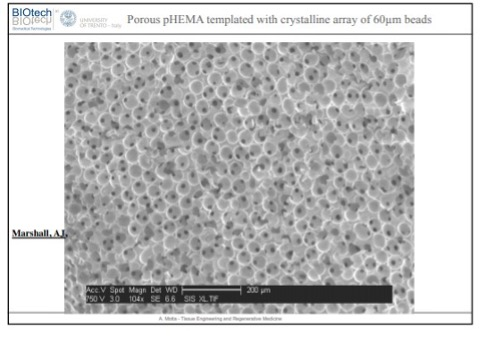
\includegraphics[width=0.5\textwidth]{pores}
\caption{\label{fig:pores}}
\end{figure}

If we analyze an image at higher magnification,  we observe that black dots measure around 5 micron. 
By playing with the scaffold, different families can be obtained. 
Results: more capillaries in the case of smaller pores. Ideal range: 40-50 microns. 
The highest vascular density was observed in the case of smaller porosity (0-100 micrometers). 
The range was explored in depth, 20 micron something appeared, the highest is around 40 micron. Very large porosity leads to the formation of a layer of endothelial cell, no 3D tube required for vascularization.  

\section{Scaffold vascularization strategies}
\begin{enumerate}
\item growth factor delivery: delivery of single or multiple angiogenic GF to stimulate. loading molecules can be performed by mixing with the polymer (fast release), include them in a drug releasing system (polymeric nanoparticle, driven by degradation time of nanoparticles ) or link the molecules to the polymeric chain. Which is the rational of the choice? It mainly depends on required timing. Strategies can be also combined in order to release our molecule at different times.
\item cell transplantation: implant EC on the tissue
\item in situ vascularisation with endogenous cells
\item scaffold pre-vascularization: pay attention to the protocol used. We must be sure that robust tubes tar produced in order to anastomize with the osteoblasts. We can also include something to attract already existing vascular tubes to the scaffold.
\item decellularised scaffold: decellularised myocardium, not populated by endothelial cells. We take a piece of myocardium, decellularize but leave the basic structure, including tube. The main difficulty in this strategy is to guarantee a very low amount of DNA (check that no debris is left after decellularization), avoid thrombogenesis through forced migration to reform endothelium.
\item angiogenic biomaterials: the best option if possible, design biomaterials able to induce vascularization per se. We can call them “precision biomaterials”, as they are designed according to have a specific function. Nature derived biomaterial: e.g. protein derived from silk, intrinsic angiogenic potential. Synthetic functionalized biomaterials.
\item microfabrication methods: top-down approach, answer to build up vessels and around them the tissue. We can bypass the issue of decellularize by directly inserting endothelial cells.
\end{enumerate}

\section{Angiogenic potential evaluations}
In vitro procedures should be carefully designed, we need to make sure that we are obtaining useful considerations on the scaffold. 
Fig \ref{fig:coculture} : seed mononuclear cells inside the hydrogel upon isolation of two main endothelial progenitor cells populations from peripheral blood.
Impact on the matrix: cells were seeded and checked after 4 and 10 days. In the case of IKVAV modified culture we have more signals. This means we have more cells, more clusters and more layers (migration). The aim was to design a precision material to be used in brain, laminin derived (brain ECM). Strategy:  isolate peptide involved in differentiation and link it to polymeric chain. 
We expect to obtain tubes in angiogenesis, but here we only observe a bunch of cells. What was wrong is the in vitro model, too far from physiology because only one layer is not good. The model was then changed: in order to reach a tube more cells are required e.g. cells able to drive tube formation -> bone marrow stem cells, which differentiate into pericytes, secrete angiogenic factors e.g. VEGF and Ang-1 and produce collagen I and IV for the ECM. 
\\
\\
\noindent
For stem cells isolated from donors we need to at least use 5 replicates, as there is a huge variability.  By applying this procedure, we can see a nice formation of tubes (well branched and interconnected) in donor 1, only pieces in donor2 and 3. Takehome message: take into consideration personalized solution in order to avoid variability and to achieve the best result. Secondly the result in co-culture was identical in terms of ECM. If the culturing conditions are good and we introduce SC, we can successfully reach vascularization.

\begin{figure}[h]
\centering
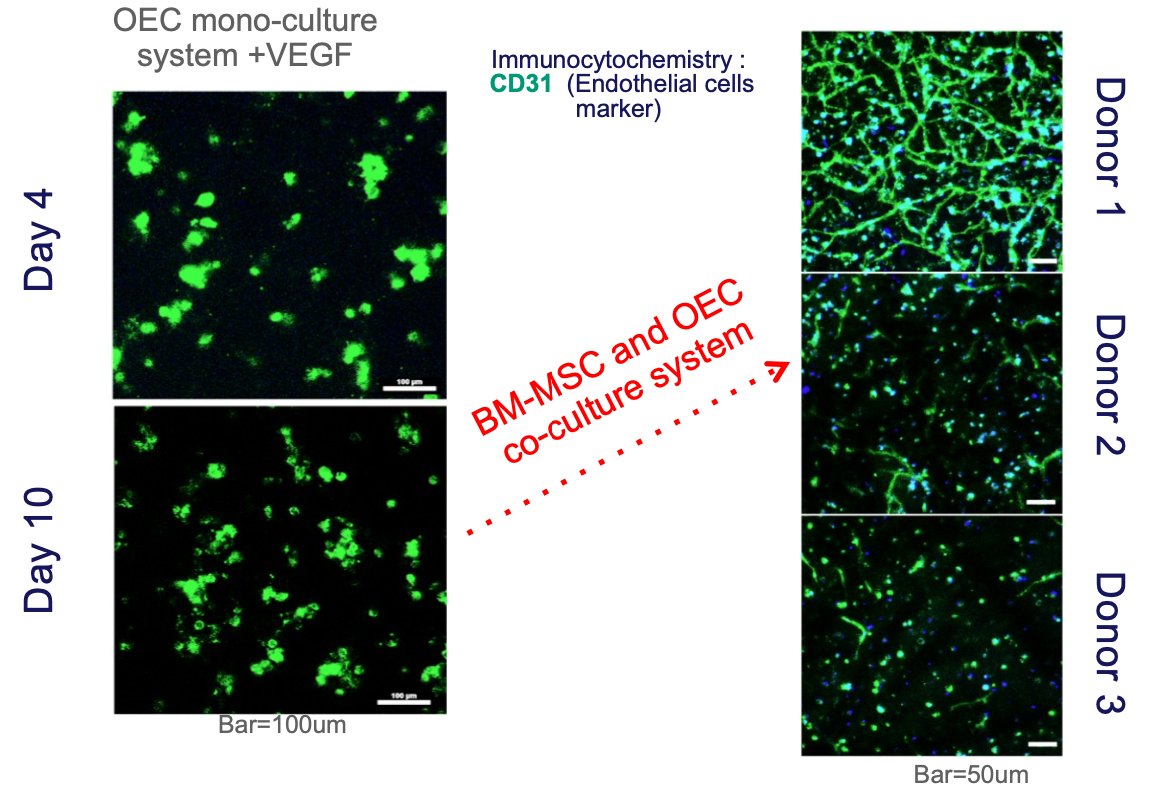
\includegraphics[width=0.5\textwidth]{coculture}
\caption{\label{fig:coculture}}
\end{figure}
\noindent
Considering the bone, the presence of two families leads to best results: osteoblast work will lead to an increase endothelial cells formation. Osteoblast cells know how much and when to release factors. Osteoblasts also produce a collagenic template used by endothelial cells to form tubes. When we take into account the scaffold, we can support the direct interaction with both osteoblast and endothelial cells. 
Example: fibroin micronet, co-cultured, 3d scaffold. The endothelial cells become tubes, there is a collagenic network.
We need that the tubes are stable. In the microscope view we can see that there is a very physiological structure. 

\section{Vascularization strategies}
New strategies to achieve better blood vessels: architecture is important, should provide something to make endothelial cell grow mechanism of angiogenesis can be amplified. Porous matrices can be loaded with growth factor, functionalization to recruit blood vessels from surrounding tissues. They should be able to penetrate and form interconnected tissue.
\\
\\
\noindent
The main vascularization strategies are:
\begin{itemize}
\item angiogenesis: ingrowth of vascular sprouts from the host microvasculature into implanted tissue construct, which finally form a new microvascular network
\item inosculation: pre-created vessels in vitro (network, not real vessels) is generated within a tissue construct prior to implantation. Connection with host vessels + already included vessels. Usually animal cells are used, in order to distinguish which vessels are new and which are implanted through staining. Sometimes scaffold tubes are not able to anastomize and die, our aim is to preserve the mixture and anastomize (circle in the picture).
\end{itemize}

\begin{figure}[h]
\centering
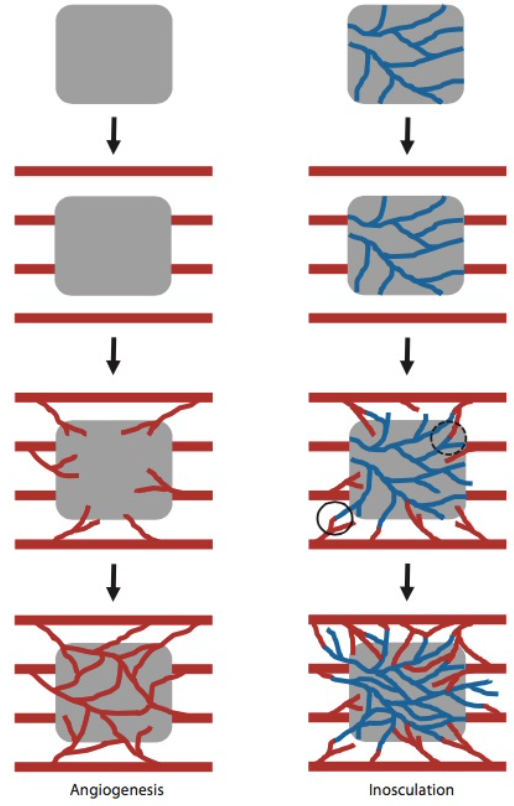
\includegraphics[width=0.3\textwidth]{vasc}
\caption{\label{fig:vasc}}
\end{figure}

\subsection{Immune response and vascularization}
We have also to remember that inflammation (immune response) induces to angiogenesis.
Initially we have the recruitment of macrophages. Granulation tissue must be vascularized.
Two different structures with different porosity. In the first case (high porosity) we have a fine granulation tissue, angiogenic factors and new vessels. After 2 weeks we have less, much less inflammatory response.  In the second case there is no vascularisation, so this is not good. There is a thick layer of fibrotic tissue.

In vivo vascularisation scaffold induced
Polymer: form a sponge with a porosity with different pore sizes. 
\begin{itemize}
\item PDLLA: blood vessels are just around (3wks)
\item PDLLAA + silk fibers: very nice capillary branch formation into the scaffold (3wks)
\end{itemize}
After 6 weeks Silk seems to be intrinsically angiogenic.
We need early and efficient angiogenesis, the winner is always the scaffold that achieves the result in a short time. Which are the intrinsic angiogenic properties of silk fibroin net and mechanism? We don’t know yet for sure, but we need them!

\begin{figure}[h]
\centering
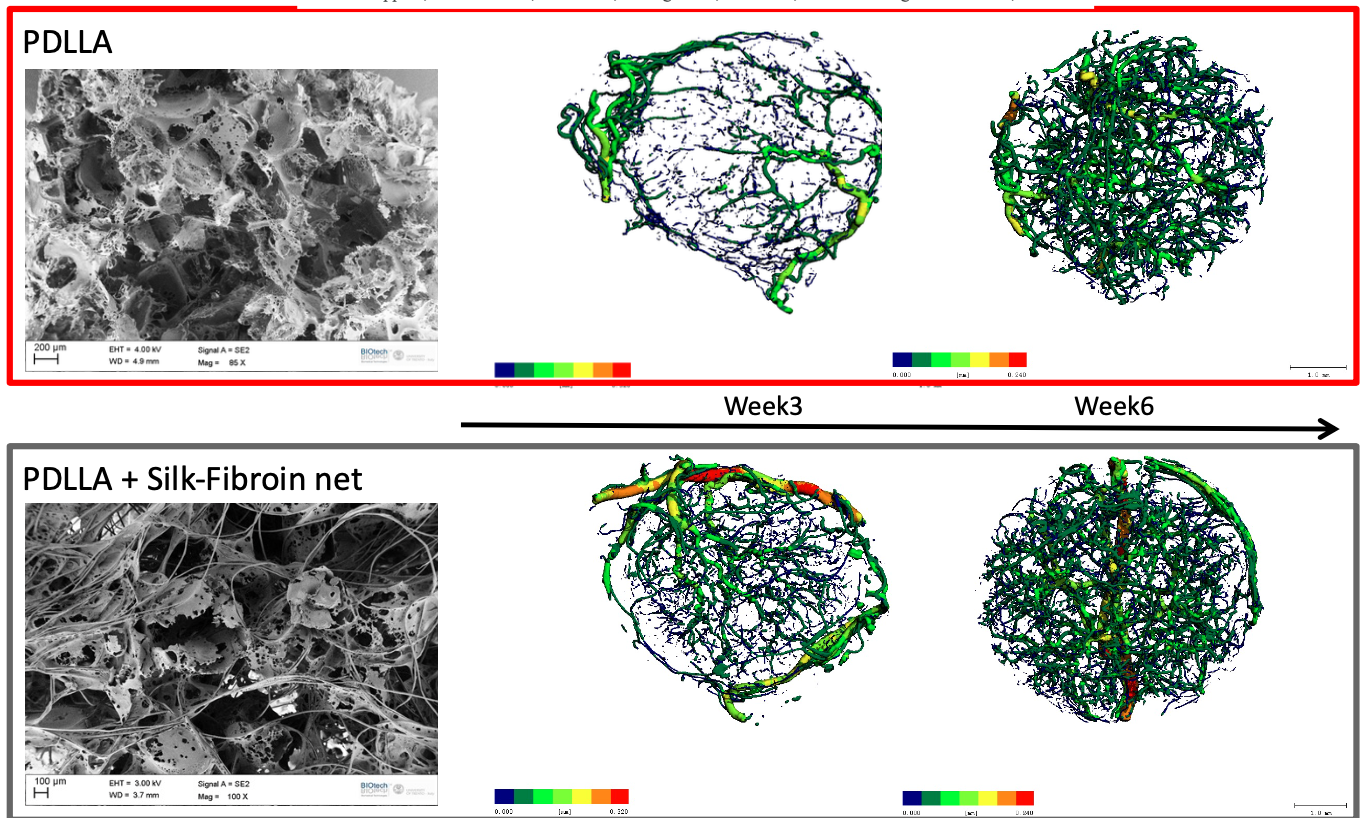
\includegraphics[width=0.5\textwidth]{pdlla}
\caption{\label{fig:pdlla}}
\end{figure}

\subsubsection{Different polymers in co-culture}
Comparison of different polymers with co-culture (HA, calcium phosphate, Ni-Ti, fibroin). The results are quite different, it’s important to carefully design the in vitro test, but it is not enough if the substrate is not specifically bioactive.

\subsubsection{Angiogenesis driven by inflammatory cells}
The fibroin net was implanted with and without pre-seeding osteoblasts. A very nice and intense angiogenesis was observes thanks to the interaction between osteoblasts and inflammatory signal.
Different pre- culture time
Manage the inflammatory response better in the case B.
Impact on angiogenesis: second scaffold has a better angiogenesis!
Drug release system works and speeds up the angiogenesis process.

\begin{figure}[h]
\centering
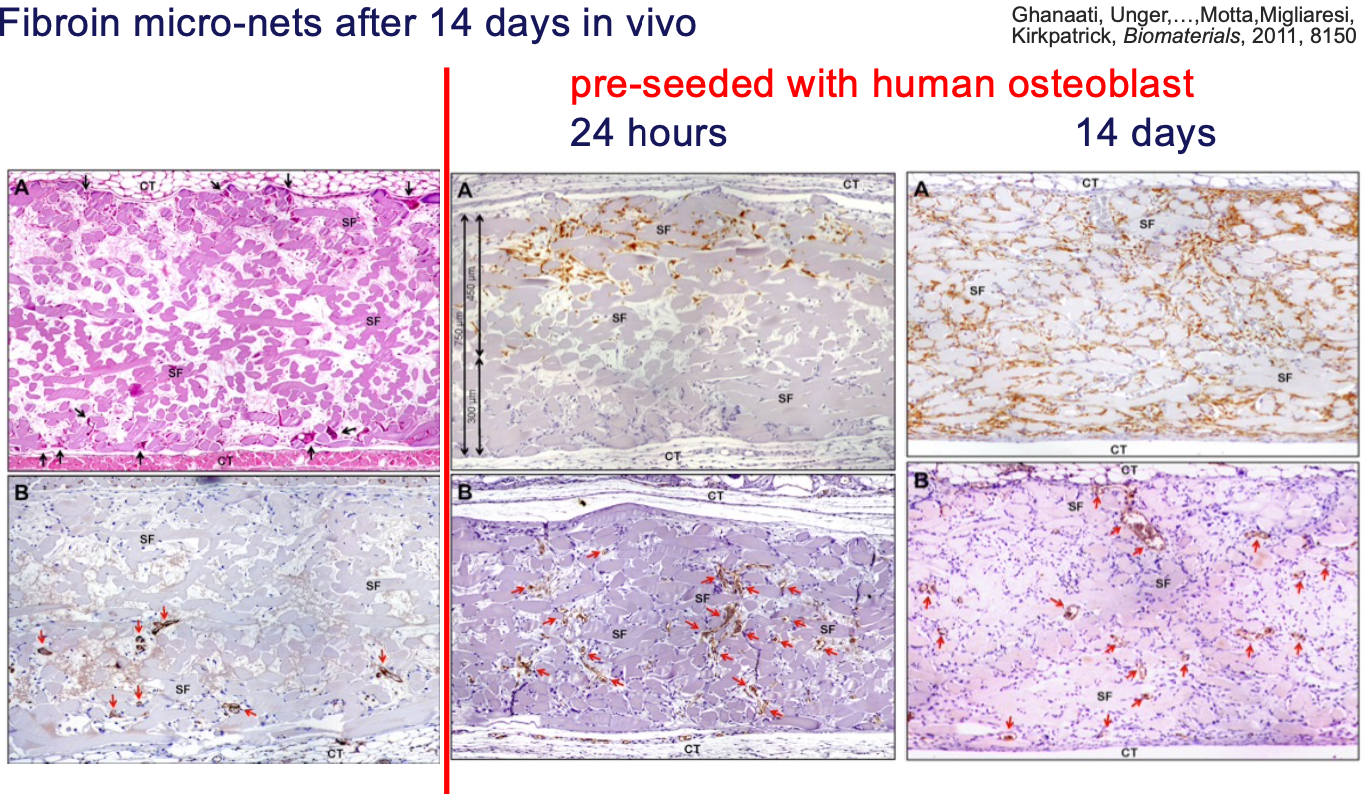
\includegraphics[width=0.5\textwidth]{fibroin}
\caption{\label{fig:fibroin}}
\end{figure}

\section{Induction of vascularization in TE scaffolds}
After the selection and dosage of the molecules we need to design how to release them into the system. 

\subsection{PDGF-containing microspheres}
Dual factor delivery from degradable scaffolds for de novo blood vessels synthesis: we can have PDGF-containing microspheres: the molecules must exit from the vescicle, move in a matrix and then release (very slow process). We need to assess degradation does not occur prior to release and whether microparticles are active and alive throughout the waiting time. 
\subsection{Cytokine delivery}
The sequential delivery of VEGF and PDGF-BB using a controlled release polymeric device subcutaneously and in hind limb ischemia model induced a mature new vascular network with vessels having a thick coat of smoot muscle cells. The combination of the two gives the best and fastest angiogenesis.
\subsection{Microparticles}
Scaffold design by microparticle assembly. Microparticles preparation:
\begin{itemize}
\item formation of microparticles via single emulsion
\item  double emulsion: with growth factors
\end{itemize}

It includes the microspheres: loaded or not with drugs.
Sintering: formation of microparticles with some porosity inside
Printing: print microparticles Single emulsion: method of sintering.

Very good adhesion with sintering process. Sintering is usually used for ? alloy, but also with polymers and ceramics.
The porosity can be improved by mixing with water (water soluble or insoluble materials).
You can also use polymers with this technology, at first this technology needed really high temperatures and so not good with polymers, but now lower temperatures are needed.

\subsection{Strategies for enhancing vascularization}
By host: with growth factors pros: easy to engineer, high quality vessels, cons: too slow
Really slow is a cons because the tissue needs to be vascularised in order to work properly.
Engineered vascular network:
pros: immediate perfusion
cons: hard to engineer, must be compatible with blood We want to provide porosity but also canals.
Also tubes can provided, for example tubes with ice, to be filled with vessels.



